\subsection{Improper Curves}

\begin{definition}
  An \emph{A-graph} (AD-HOC TERM, THINK OF A BETTER NAME)
is a graph $G$ together with a Jordan curve/arc $C$ that intersects
every edge of $C$ in exactly one point, possibly an endpoint,
and where every vertex on $C$ has at least one incident edge on each side.
\end{definition}

They have the following properties:

\begin{enumerate}
\item Every face, including the outer face, is a quadrilateral or a
  triangle.
\item Every $v$ vertex on $C$ is incident to precisely two triangles,
  one 
above $v$ and one below $v$. (This holds also when $v$ is a boundary
vertex; in this case, one of the triangles is the other face.)
\item Every triangle face contains one vertex on $C$, one vertex in
  $L$ and one vertex in $R$.
\item Every vertex is incident to at least two edges.
\item Every vertex on $C$ is incident to at least three edges.
EXCEPTION: If $v$ is on the outer face, it can have degree 2.
WE MUST EXCLUDE THE DEGREE-2 CASE SOMEWHERE. IT IS TRIVIAL TO HANDLE.
I DON'T KNOW WHERE THE PROPER PLACE FOR HANDLING IT.
\end{enumerate}

\begin{thm}\thmlabel{a-graph}
(Generalization of \thmref{quad})

   Let
   \begin{compactenum}
     \item  $G$ be an A-graph;
     \item  $C:[0,1]\to\R^2$ be an admissible Jordan curve for $T$;
     \item $r_1,\ldots,r_k \subseteq E(V)\cup E(G)$ be the sequence of vertices and open edges
           of $T$ that are intersected by $C$, in the order
           that they are intersected by $C$;
     \item $y_1<\cdots<y_k$ be any sequence of numbers; and
     \item .... [$\Delta$ be a triangle that is compatible with 
           $r_1,\ldots,r_m$ and $y_1,\ldots,y_m$.]
  \end{compactenum}
$G$ has a
   \Fary\ embedding in which the outer face $f$ [ is $\Delta$ ]
   and, for each $i\in\{1,\ldots,k\}$, 
   \begin{compactenum}
       \item if $r_i$ is a vertex, then $r_i$ is drawn on the y-axis, with y-coordinate $y_i$;
%       \item if $r_i$ is an edge contained in $C$, then $r_i$ is drawn so that
%         it is contained in the y-axis; or
       \item If $r_i$ is an edge whose intersection with $C$ is a
         single point interior to $r_i$, 
         the intersection of $r_i$ with the
         y-axis has y-coordinate
         $y_i$.
   \end{compactenum}
\end{thm}

\begin{proof}
  We will describe the straight-line embedding by assigning a slope $s_e$
to every edge $e\in E$.
Since there can be no vertical edges, the slopes are well-defined.
We have $m=|E|$ slope variables.

Since every edge goes through a point on the y-axis with known
coordinate, the slope fixes the line through the edge.
 Since
every vertex not on $C$ is incident to at least two edges that go
through
distinct points on the y-axis, location of such a vertex is fixed.

A necessary condition for the slopes is that the lines of edges that
go through a common vertex should be concurrent:
We can extend the function $y$ to all edges, independently of how they
intersect $C$. If $e$ intersects $C$ at an endpoint, we let $y_e$ be
the
given $y$-coordinate of that endpoint. THINK ABOUT A BETTER NOTATION!
%
Let $v$ be a vertex $v$ not on $C$, and let $e_i, e_j, e_k$ be three
edges incident to $v$.
The fact that the three supporting lines of $e_i$, $e_j$, and $e_k$ 
meet at a common point (the location of $v$) is expressed
the following \emph{concurrency constraint} 
in terms of the slopes $s_i,s_j,s_k$:
\begin{equation}\eqlabel{slope} 
\left|
  \begin{matrix}
    1&1&1\\
s_i&s_j&s_k\\
y_i&y_j&y_k
  \end{matrix}
\right|=
   ({y_j-y_k}) s_i + ({y_k-y_i}) s_j 
          + ({y_i-y_j})s_k  = 0
\end{equation}
Since $y_1,\ldots,y_m$ are given, this is a linear equation
in $s_1,\ldots,s_m$.
Writing this equation for all triplets of edges incident to a common
vertex will include many redundant equations.
If $d_v$ edges meet in a vertex~$v$, 
 It suffices to take $d_v-2$ equations: We choose two fixed
incident edges $e_i$ and $e_j$ and run $e_k$ through the remaining
$d-2$ edges, specifying that $e_k$ should go through the common vertex
of $e_i$ and $e_j$.

It will be important to have as many equations as variables;
thus, we add some more equations for the edges that emanate from a
vertex on $C$.
Suppose that edges $a_1,\ldots,a_k$ and $b_1,\ldots,b_l$ go to the
right, from bottom to top.
We have $k,l\ge1$ and $k+l\ge 3$.
Let us first look at the slopes on the right side.
We want these slopes to be increasing:
$s_{b_1} < s_{b_2} < \dots  <s_{b_l}$. We stipulate a stronger
condition:
We require that the slopes
$s_{b_2}, \dots, s_{b_{l-1}}$ partition the interval
$[s_{b_1},s_{b_l}]$ in fixed proportions. In other words
\begin{equation}
  \label{eq:proportion}
s_{b_i} = s_1 + \lambda_i(s_{b_{l}}-s_{b_1}),
\end{equation}
for some fixed sequence $0<\lambda_2<\cdots<\lambda_{l-1}<1$.
(For example, we might set $\lambda_i := i/(l-1)$.)
This gives $l-2$ equations, for $l\ge 2$. Similarly, we get
$k-2$ equations for the slopes
$s_{a_1}, \dots, s_{a_{k}}$ on the left side, for $k\ge 2$.
In addition, for $k,l\ge 2$, we require that the \emph{range} of
slopes
on the two sides are in a fixed proportion
\begin{equation}
  \label{eq:proportion2}
s_{a_1}-s_{a_{k}} = \mu (s_{b_{l}}-s_{b_1}),
\end{equation}
for some fixed value $\mu>0$.

This leads to $(k+l)-3$ equations in total.


 \figref{proportional}


The notations
$\lambda_i$ and 
$\mu$ are here used in a local sense; for a different vertex $v$, we may
choose different constants.
\begin{figure}
     \centering{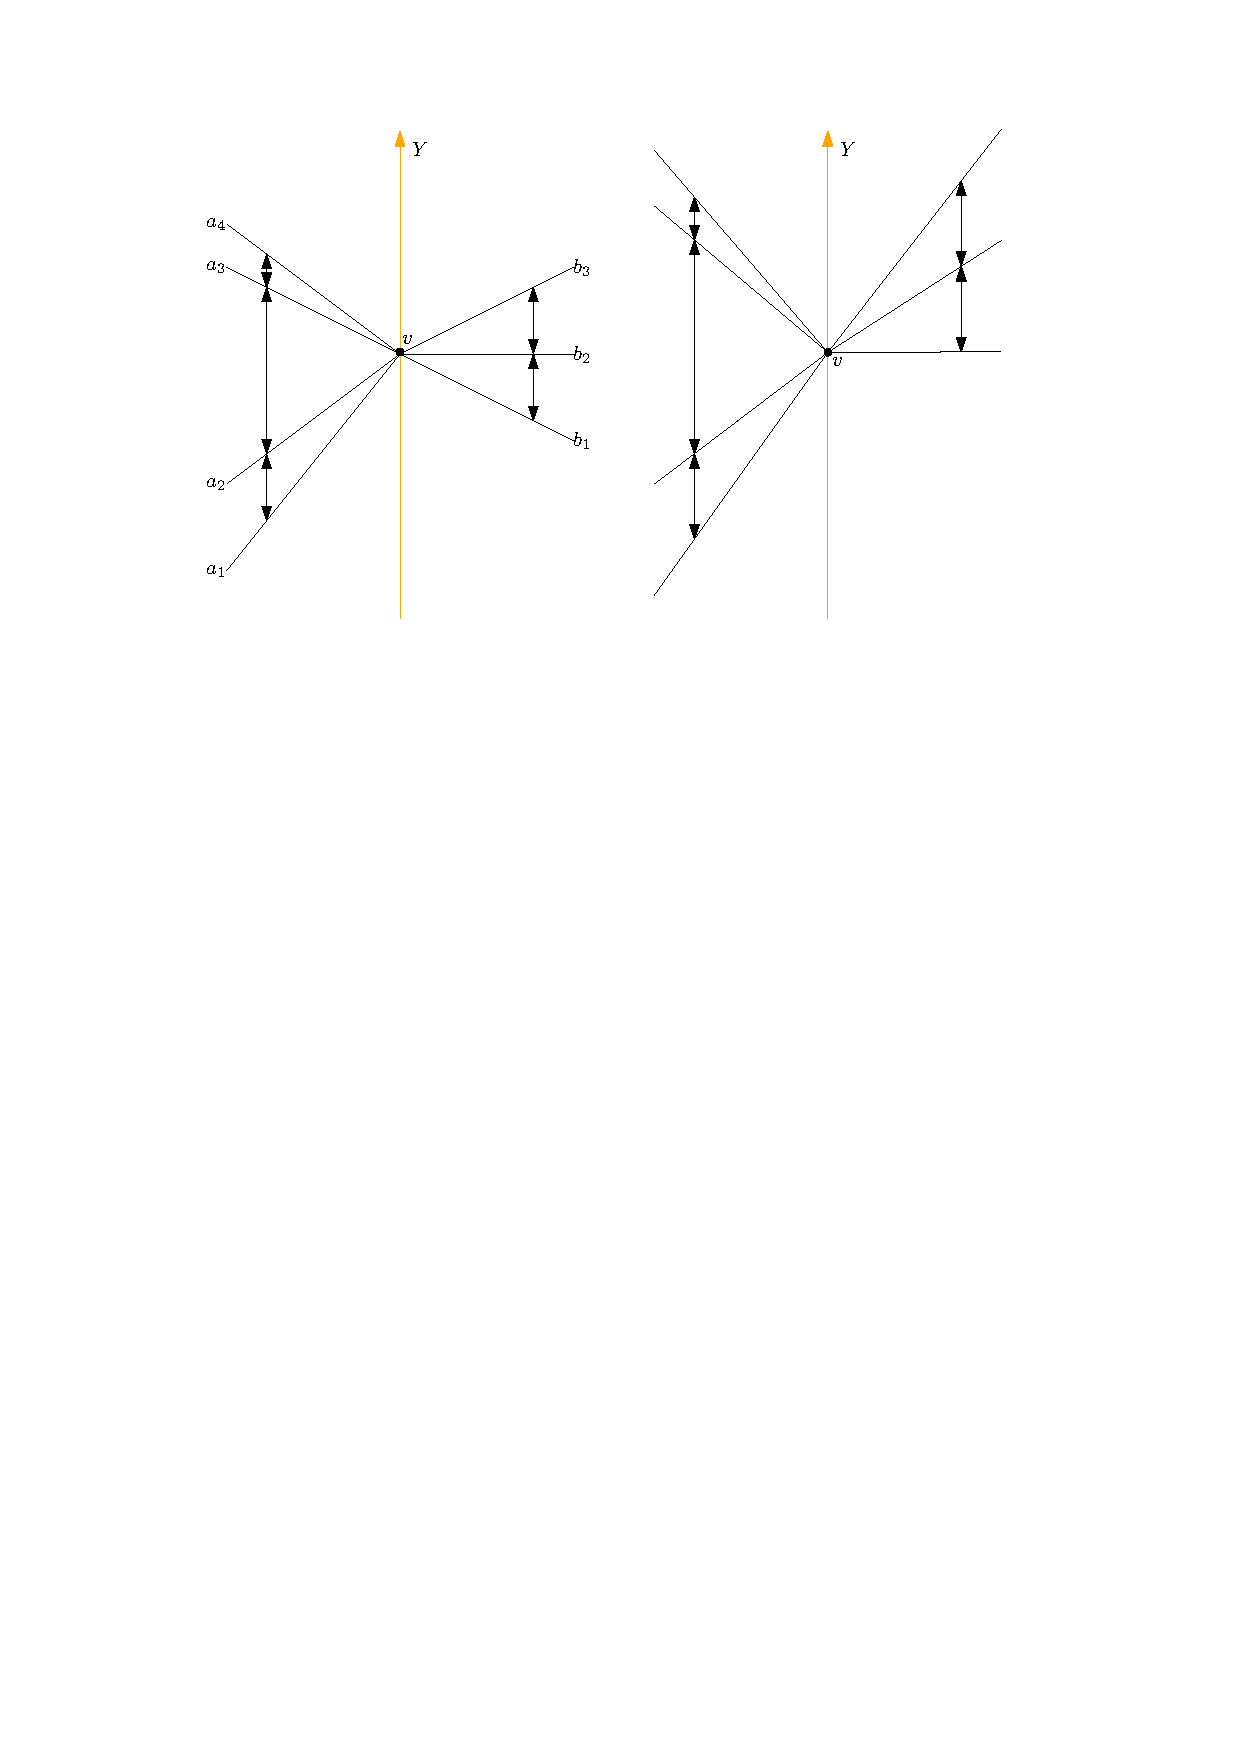
\includegraphics{figs/proportional}}
     \caption{The proof of \lemref{partition}.}
     \figlabel{proportional}
  \end{figure}
The total number
 

  The total number of equations is therefore
\begin{equation}
  \label{eq:number-equations2}
  \sum_{v=1}^n(d_v-2) = 2m-2n = m-4,
\end{equation}
using the relation $m=2n-4$ for quadrangulations, which follows from
Euler's formula.


 We have four more equations for the specified slopes
$s_1, s_a, s_b, s_m$.


\end{proof}



%%% Local Variables:
%%% mode: latex
%%% TeX-master: "freecoll"
%%% End:
